\documentclass[en]{../../../../../../eplexam}

\newcolumntype{M}[1]{>{\raggedright}m{#1}}

\hypertitle{Instrumentation and Sensors}{7}{ELEC}{2811}{2019}{Janvier}{All}
{Alice Borbath \and Martin Braquet \and Olivier Leblanc}
{David Bol and Laurent Francis}

Evaluation marks:
\begin{itemize}
    \item Two reports: 4/20
    \item Final report: 8/20
    \item Exam: 5/20 for the 14 questions and 3/20 for the open question about the project
\end{itemize}


\section{}

For each of the following sensors, choose if it is a direct or an indirect sensor:

\begin{itemize}
    \item A posistor
    \item A piezoresistor
    \item A capacitive accelerometer
    \item A chemical-based hygristor
    \item 
\end{itemize}

\nosolution

\section{}

As regards a piezoresistance with a strain gauge, select the \textbf{false} proposition:

\begin{itemize}
    \item The strain gauge factor of the silicium highly depends on its doping.
    \item The strain gauge factor for metals can vary over large values between $-120$ and 200.
    \item The strain gauge factor depends on the Poisson's coefficients and the relative variation of the resistivity with the stress.
    \item The strain gauge factor measures the ratio between the relative variation of the resistance and the strain.
    \item 
\end{itemize}


\nosolution

\section{}

Give four oscillators and their type (sine or binary).


\nosolution

\section{}

Give three applications based on the piezoelectric effect.


\nosolution

\section{}

We consider the general configuration of a Sallen--Key filter.

\begin{figure}[H]
    \centering
    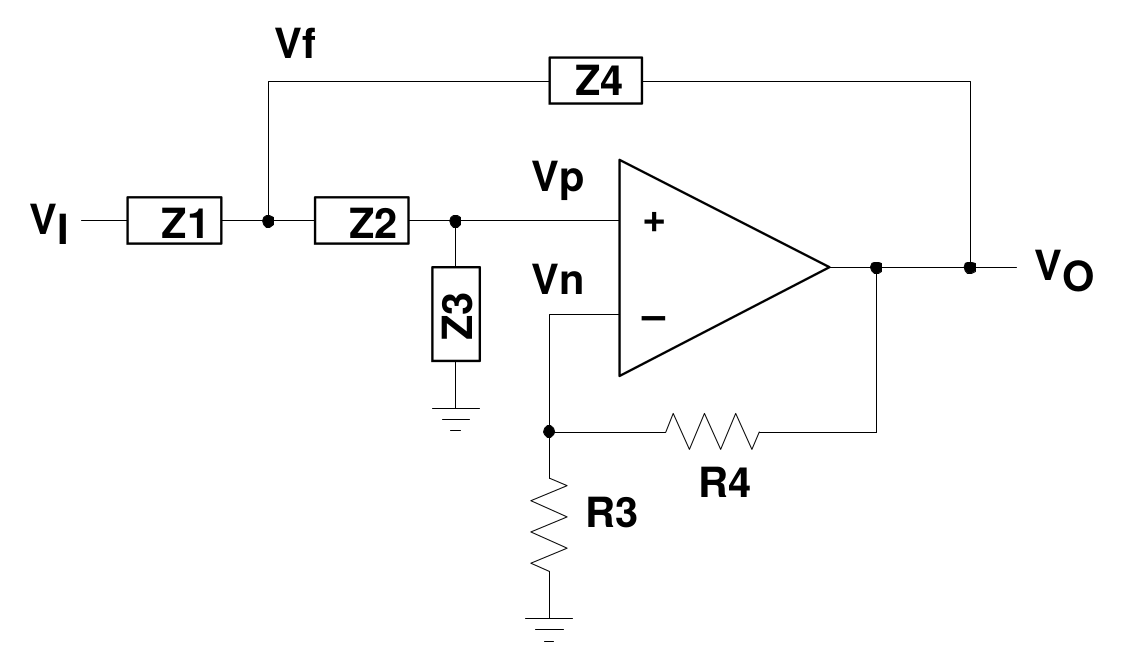
\includegraphics[width=0.5\textwidth]{sallen.png}
\end{figure}

For each statement, select true or false: 100 \% for a right answer, 0 \% for no answer and $-50$ \% for a wrong answer.

\begin{itemize}
    \item When $Z_1$ and $Z_2$ are capacitors and $Z_3$ and $Z_4$ are resistors, it is a high pass filter.
    \item The gain depends on the impedances $Z_1$ to $Z_4$.
    \item This filter is always used for sensors with a changing resistance.
    \item The Sallen--Key filter is considered as a second order filter.
\end{itemize}

\nosolution


\section{}

As regards capacitive sensors, select the \textbf{false} proposition:

\begin{itemize}
    \item The relation between the capacitance and the stimulus is always linear in a capacitor with parallel plates.
    \item The measurement of the water level in a tank with a variable capacitor must come with a temperature measurement.
    \item A capacitor has a linear relation with humidity.
    \item 
    \item 
\end{itemize}

\nosolution


\section{}

A team of engineers is asked to measure leakages of hydrogen in order to estimate the risk of explosion. Leakage of hydrogen becomes dangerous when the concentration in air reaches 4 \% since it associates with oxygen and it results in an explosion.  The hydrogen is stored in a room where other bottles of gases can be placed, mostly carbon monoxide and ammonia. 

Do you recommend them to use the MOX gas sensor for their project? Give arguments based on the characteristic below (sensitivity, offset, calibration, selectivity, limit of concentration) and the working of the MOX gas sensor.

\begin{figure}[H]
    \centering
    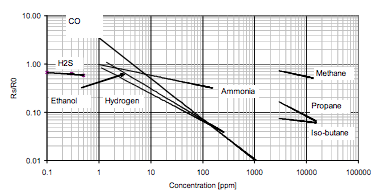
\includegraphics[scale=0.6]{quest7.png}
    \caption{Characteristic of the MOX gas sensor}
\end{figure}

\nosolution


\section{}

You can read hereunder one possible classification of inaccuracies. For each compartment, give an example as well as a possible way to reduce its effect.

\begin{table}[H]
    \centering
    \begin{tabular}{|M{4.5cm}|M{7cm}|}
        \hline
         Systematic inaccuracy common to all sensors &                                       \\
         \hline
         Stochastic inaccuracy from one sensor to another &                              \\
         \hline
         Stochastic inaccuracy in the same sensor &                              \\
         \hline
    \end{tabular}
\end{table}

\nosolution


\section{}

Select the right answer: 100 \% for a right answer, 0 \% for no answer and $-50$ \% for a wrong answer.

\begin{itemize}
    \item The amplitude distribution of the white noise is:
    \begin{center}
        gaussian - constant
        \end{center}
    \item The $1/f$ trend in the frequency domain is associated with:
    \begin{center}
    flicker noise - environmental noise
    \end{center}
    \item The integral non-linearity is related to gain errors.
    \begin{center}
        True - False
    \end{center}
    \item Oversampling allows to relax the roll-off factor of the filter.
    \begin{center}
        True - False
    \end{center}
\end{itemize}

\nosolution


\section{}

What is the concept represented by the double arrow? Explain what it is and how to compute it. What are the signals $s_1$ and $s_0$?

\begin{figure}[H]
    \centering
    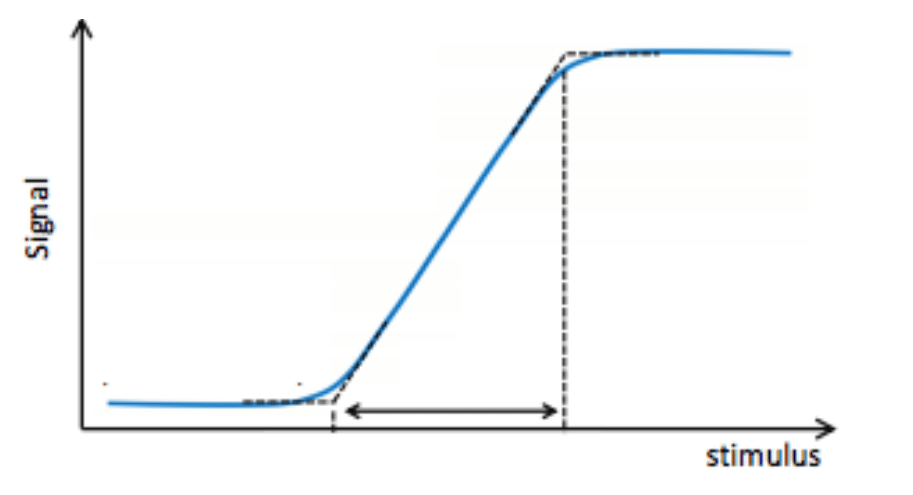
\includegraphics[width=0.6\textwidth]{quest11.png}
\end{figure}

\nosolution


\section{}

Give the input-referred noise of this system. (The pressure sensor has a gain $A_{\textnormal{conv}}$ and the amplificator, a gain $A_{\textnormal{v}}$.)

\begin{figure}[H]
    \centering
    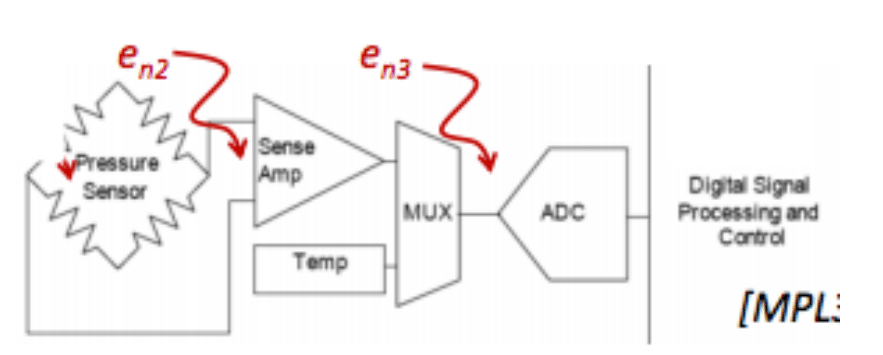
\includegraphics[width=0.6\textwidth]{quest12.png}
\end{figure}

\nosolution


\section{}

HDR CMOS images: resolution enhancement.

We aim to use resolution enhancement on dark and bright pixels to improve the quality of our image, explain how you would achieve this.

\begin{figure}[H]
    \centering
    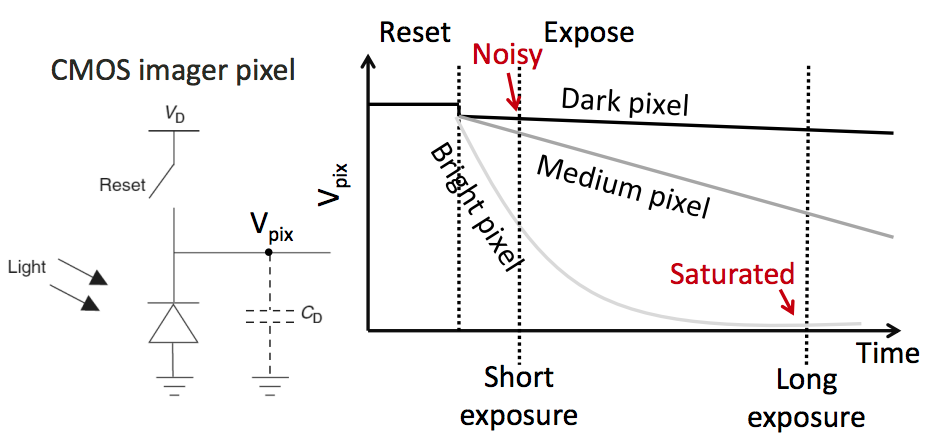
\includegraphics[scale=0.45]{quest13.png}
\end{figure}

\nosolution


\section{}

A periodic noise signal of frequency 50 Hz is added on the signal to detect, which is sampled at 500 S/s. How can you reduce this noise with a digital filter? Which filter is the best for this application? Why? Explain how it works.

\nosolution


\section{Question about the project}

We had to take the height of the liquid in the glass into account, which was not the case during the project.

We suppose we stay at constant ambient weather conditions, s.t. the temperature and relative humidity don't have to be taken into account. We use the same glass of height $h_{\textnormal{glass}} = 15$ cm.
\[
    R_s = R_0 \left[1-\alpha \left(\frac{h_{\textnormal{liquid}}}{h_{\textnormal{glass}}}\right)^2\right]\,.
\]

\begin{center}
\begin{tabular}{|c|c|}
\hline
    Type & $ \alpha $ \\
    \hline
     Maes Raedler & 0.1 \\
     \hline
     Jupiler & 0.4 \\
     \hline
     Taras Boulba & 0.5 \\
     \hline
     Grimbergen & 0.7 \\
     \hline 
     Rochefort & 0.9 \\
     \hline
\end{tabular}
\end{center}

First, we suppose that we serve each drink, at the same height and in the same type of glass.

\begin{enumerate}
    \item $R_0$ has an unknown value between 0.1 and 150 k$\Omega$. Gain sensitivity $0.1$ mV$/\Omega$. The addition of white noise, quantization error, device-to-device variation, etc. is resumed in an overall amplitude error of $0.2$ mV. Compute the minimum height of liquid $h_{\textnormal{liquid}}$ in order to be able to separate the Jupiler from the Taras Boulba.

    Now, we want to remove the need of having the same height of liquid for the different drinks. But we still assume it varies in a span from 80 mm to 120 mm.
    
    \item Knowing the distance $d=h_{\textnormal{glass}} - h_{\textnormal{liquid}}$, explain how you could introduce it in your project.
    Start by giving a summary of your actual system, your whole system.
    
    \item 
    
    \item Give a sensor that could be used to measure this distance.
    
\end{enumerate}
\nosolution
\end{document}
